\subsection{Experimental setup}
\label{sec:setup}

\subsubsection{System}
\label{sec:system}

For our experiments, we use a server that has an x86-based 64 core AMD EPYC-7742 processor. This processor has a clock frequency of $2.25$ GHz and $512$ GB of DDR4 system memory. Each core has an L1 cache of $4$ MB, an L2 cache of $32$ MB, and a shared L3 cache of $256$ MB. The machine uses Ubuntu 20.04.


\subsubsection{Configuration}
\label{sec:configuration}

We use 32-bit unsigned integer for vertex IDs, 32-bit floating point for edge weights, but use 64-bit floating point for hashtable values, total edge weight, modularity calculation, and all places where performing an aggregation/sum of floating point values. Affected vertices are represented with an 8-bit integer vector. Computing the weighted degree of each vertex, the local moving phase, and aggregating the edges for the super-vertex graph, employ OpenMP's \textit{dynamic schedule} with a chunk size of $2048$ for dynamic workload balancing among threads. We set the iteration tolerance $\tau$ to $10^{-2}$, the tolerance drop per pass $TOLERANCE\_DECLINE\_FACTOR$ to $10$ (threshold-scaling optimization), maximum number of iterations per pass $MAX\_ITERATI$ $ONS$ to $20$, and the maximum number of passes $MAX\_PASSES$ to $10$ \cite{sahu2023gvelouvain}. Further, we set the aggregation tolerance $\tau_{agg}$ to $0.8$ for large (static) graphs with generated random batch updates, but keep it disabled, i.e., set $\tau_{agg}$ to $1$, for real-world dynamic graphs. Unless mentioned otherwise, we execute all parallel implementations with a default of $64$ threads (to match the number of cores available on the system). We use GCC 9.4 and OpenMP 5.0 \cite{openmp18} for compilation.


\subsubsection{Dataset}
\label{sec:dataset}

To experiment with real-world dynamic graphs, we employ five temporal networks sourced from the Stanford Large Network Dataset Collection \cite{snapnets}, detailed in Table \ref{tab:dataset}. Here, the number of vertices range from $24.8$ thousand to $2.60$ million, temporal edges from $507$ thousand to $63.4$ million, and static edges from $240$ thousand to $36.2$ million. For experiments involving large static graphs with random batch updates, we utilize $12$ graphs as listed in Table \ref{tab:dataset-large}, obtained from the SuiteSparse Matrix Collection \cite{suite19}. Here, the number of vertices in the graphs varies from $3.07$ to $214$ million, and the number of edges varies from $25.4$ million to $3.80$ billion. With each graph, we ensure that all edges are undirected and weighted with a default weight of $1$.

\begin{table}[hbtp]
  \centering
  \caption{List of $13$ graphs obtained SuiteSparse Matrix Collection \cite{suite19} (directed graphs are marked with $*$). Here, $|V|$ is the number of vertices, $|E|$ is the number of edges (after adding reverse edges), $D_{avg}$ is the average degree, and $|\Gamma|$ is the number of communities obtained using Louvain algorithm.\ignore{In the table, B refers to a billion, M refers to a million and K refers a thousand.}}
  \label{tab:dataset}
  \begin{tabular}{|c||c|c|c|c|}
    \toprule
    \textbf{Graph} &
    \textbf{\textbf{$|V|$}} &
    \textbf{\textbf{$|E|$}} &
    \textbf{\textbf{$D_{avg}$}} &
    \textbf{\textbf{$|\Gamma|$}} \\
    % \textbf{$1 - \Gamma_G$} \\
    \midrule
    \multicolumn{5}{|c|}{\textbf{Web Graphs (LAW)}} \\ \hline
    indochina-2004$^*$ & 7.41M & 341M & 41.0 & 4.24K \\ \hline  % & \num{4.7e-4} & 2.9 GB
    uk-2002$^*$ & 18.5M & 567M & 16.1 & 42.8K \\ \hline  % & \num{9.6e-5} & 16 GB
    arabic-2005$^*$ & 22.7M & 1.21B & 28.2 & 3.66K \\ \hline  % & \num{5.5e-4} & 11 GB
    uk-2005$^*$ & 39.5M & 1.73B & 23.7 & 20.8K \\ \hline  % & \num{9.6e-5} & 16 GB
    webbase-2001$^*$ & 118M & 1.89B & 8.6 & 2.76M \\ \hline  % & \num{7.3e-7} & 18 GB
    it-2004$^*$ & 41.3M & 2.19B & 27.9 & 5.28K \\ \hline  % & \num{3.8e-4} & 19 GB
    sk-2005$^*$ & 50.6M & 3.80B & 38.5 & 3.47K \\ \hline  % & \num{5.8e-4} & 33 GB
    \multicolumn{5}{|c|}{\textbf{Social Networks (SNAP)}} \\ \hline
    com-LiveJournal & 4.00M & 69.4M & 17.4 & 2.54K \\ \hline  % & \num{7.9e-4} & 480 MB
    com-Orkut & 3.07M & 234M & 76.2 & 29 \\ \hline  % & \num{6.7e-2} & 1.7 GB
    \multicolumn{5}{|c|}{\textbf{Road Networks (DIMACS10)}} \\ \hline
    asia\_osm & 12.0M & 25.4M & 2.1 & 2.38K \\ \hline  % & \num{8.4e-4} & 200 MB
    europe\_osm & 50.9M & 108M & 2.1 & 3.05K \\ \hline  % & \num{6.6e-4} & 910 MB
    \multicolumn{5}{|c|}{\textbf{Protein k-mer Graphs (GenBank)}} \\ \hline
    kmer\_A2a & 171M & 361M & 2.1 & 21.2K \\ \hline  % & \num{9.4e-5} & 3.2 GB
    kmer\_V1r & 214M & 465M & 2.2 & 6.17K \\ \hline  % & \num{3.2e-4} & 4.2 GB
  \bottomrule
  \end{tabular}
\end{table}
% We convert directed graphs (marked with $*$) to undirected by duplicating edges in the reverse direction, and set the weight of each edge to $1$. and $F_{size}$ is size of the \textit{MatrixMarket} file

\begin{table}[hbtp]
  \centering
  \caption{List of $12$ graphs obtained from the SuiteSparse Matrix Collection \cite{suite19} (directed graphs are marked with $*$). Here, $|V|$ is the total number of vertices, $|E|$ is the total number of edges (after making the graph undirected), and $|\Gamma|$ is the number of communities obtained using \textit{Static Louvain} \cite{sahu2023gvelouvain}.}
  \label{tab:dataset-large}
  \begin{tabular}{|c||c|c|c|}
    \toprule
    \textbf{Graph} &
    \textbf{\textbf{$|V|$}} &
    \textbf{\textbf{$|E|$}} &
    \textbf{\textbf{$|\Gamma|$}} \\
    \midrule
    \multicolumn{4}{|c|}{\textbf{Web Graphs (LAW)}} \\ \hline
    indochina-2004$^*$ & 7.41M & 341M & 4.24K \\ \hline
    arabic-2005$^*$ & 22.7M & 1.21B & 3.66K \\ \hline
    uk-2005$^*$ & 39.5M & 1.73B & 20.8K \\ \hline
    webbase-2001$^*$ & 118M & 1.89B & 2.76M \\ \hline
    it-2004$^*$ & 41.3M & 2.19B & 5.28K \\ \hline
    sk-2005$^*$ & 50.6M & 3.80B & 3.47K \\ \hline
    \multicolumn{4}{|c|}{\textbf{Social Networks (SNAP)}} \\ \hline
    com-LiveJournal & 4.00M & 69.4M & 2.54K \\ \hline
    com-Orkut & 3.07M & 234M & 29 \\ \hline
    \multicolumn{4}{|c|}{\textbf{Road Networks (DIMACS10)}} \\ \hline
    asia\_osm & 12.0M & 25.4M & 2.38K \\ \hline
    europe\_osm & 50.9M & 108M & 3.05K \\ \hline
    \multicolumn{4}{|c|}{\textbf{Protein k-mer Graphs (GenBank)}} \\ \hline
    kmer\_A2a & 171M & 361M & 21.2K \\ \hline
    kmer\_V1r & 214M & 465M & 6.17K \\ \hline
  \bottomrule
  \end{tabular}
\end{table}



\subsubsection{Batch generation}
\label{sec:batch-generation}

For experiments involving real-world dynamic graphs, we first load $90\%$ of the temporal edges of each graph from Table \ref{tab:dataset}, and ensure that all edges are weighted with a default weight of $1$, and that they are undirected by adding the reverse edges. Subsequently, we load $B$ edges in $100$ batch updates. Here, $B$ denotes the desired batch size, specified as a fraction of the total number of temporal edges $|E_T|$ in the graph, and ensure that the batch update is undirected. For experiments on large graphs with random batch updates, we take each base graph from Table \ref{tab:dataset-large} and generate random batch updates \cite{com-zarayeneh21} comprising an $80\% : 20\%$ mix of edge insertions and deletions to emulate realistic batch updates, each with an edge weight of $1$. To prepare the set of edges for insertion, we select vertex pairs with equal probability. For edge deletions, we remove the desired number of existing edges, with equal probability of selecting each edge. To simplify, we ensure no new vertices are added or removed from the graph. The batch size is measured as a fraction of edges in the original graph, ranging from $10^{-7}$ to $0.1$ (i.e., $10^{-7}|E|$ to $0.1|E|$), with multiple batches generated for each size for averaging. For a billion-edge graph, this amounts to a batch size of $100$ to $100$ million edges.\ignore{Keep in mind that dynamic graph algorithms are helpful for small batch sizes in interactive applications. For large batches, it is usually more efficient to run the static algorithm.} All batch updates are undirected, i.e., for every edge insertion $(i, j, w)$ in the batch update, the edge $(j, i, w)$ is also a part of the batch update. We employ five distinct random batch updates for each batch size, and report average across these runs in our experiments.


\subsubsection{Measurement}
\label{sec:measurement}

We evaluate the runtime of each approach on the entire updated graph, including the local-moving phase, aggregation phase, the initial and incremental marking of affected vertices, convergence detection, and all the necessary intermediary steps, but excluding only the initial memory allocation/deallocation time. We assume that the total edge weight of the graphs is known, and can be tracked upon each batch update.

\begin{figure*}[!hbt]
  \centering
  \subfigure[Overall Runtime]{
    \label{fig:temporal-summary--runtime-overall}
    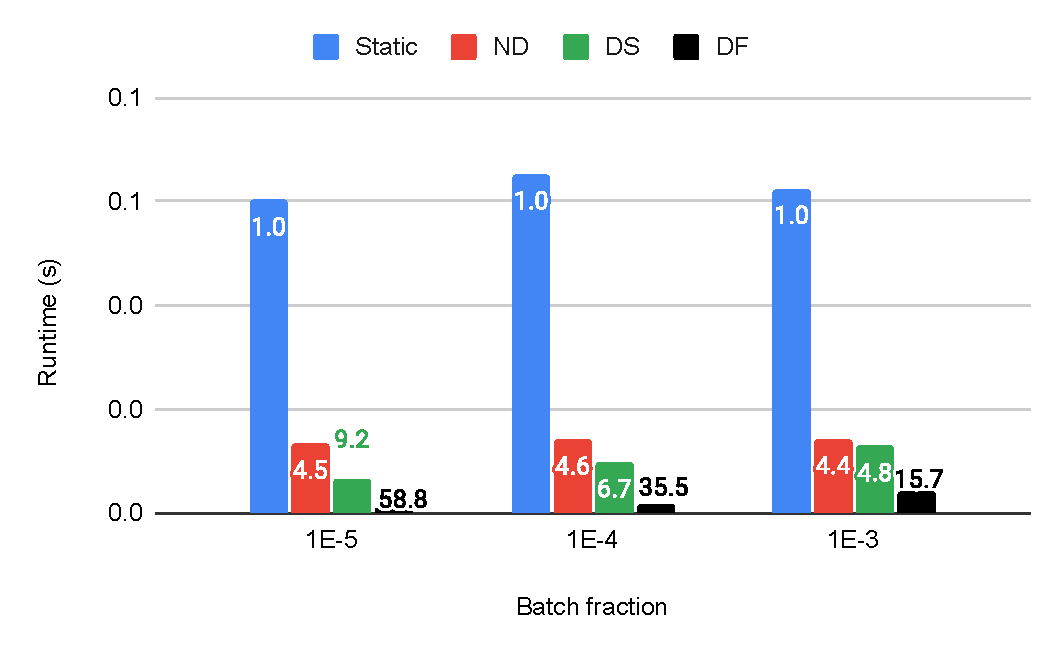
\includegraphics[width=0.48\linewidth]{out/temporal-summary-runtime-overall.pdf}
  }
  \subfigure[Overall Modularity of communities obtained]{
    \label{fig:temporal-summary--modularity-overall}
    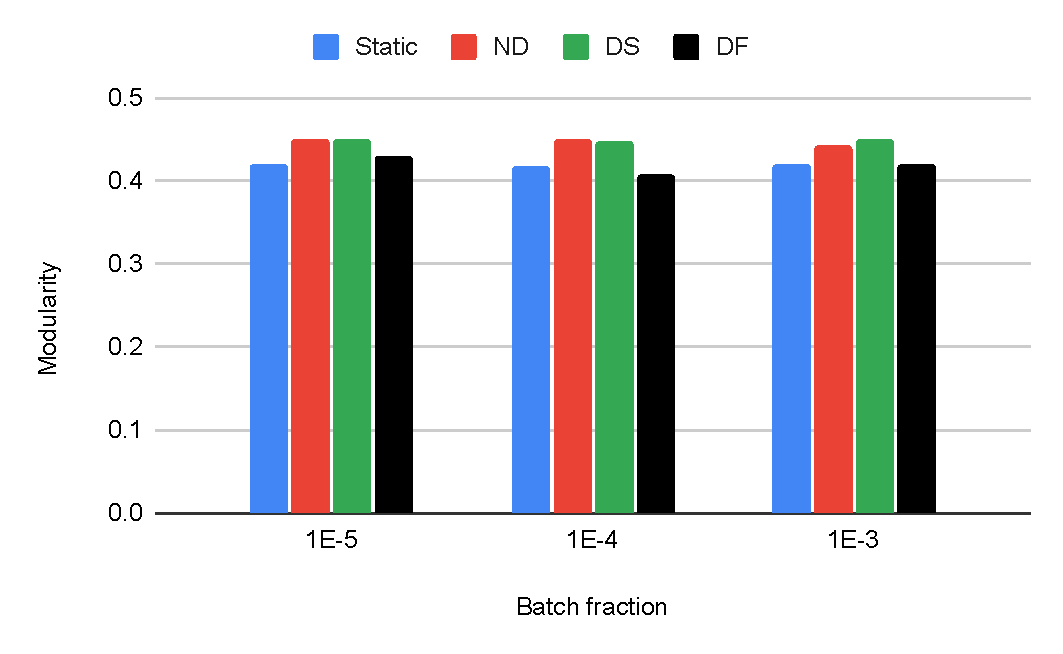
\includegraphics[width=0.48\linewidth]{out/temporal-summary-modularity-overall.pdf}
  } \\[2ex]
  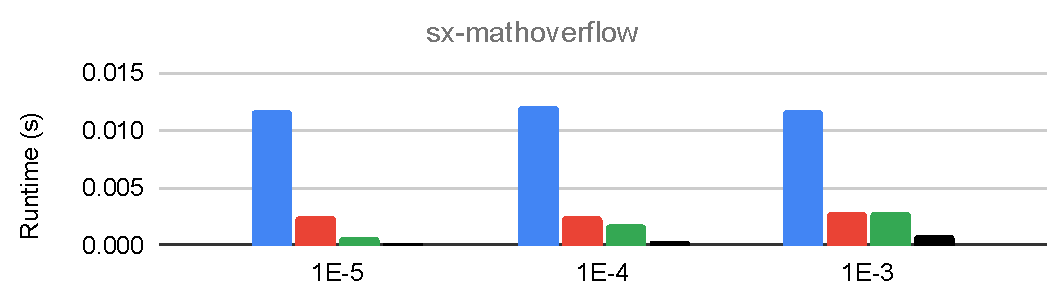
\includegraphics[width=0.48\linewidth]{out/temporal-summary-runtime-sx-mathoverflow.pdf}
  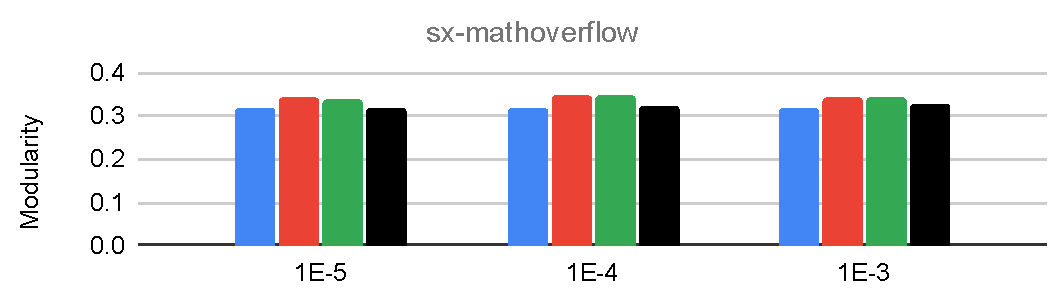
\includegraphics[width=0.48\linewidth]{out/temporal-summary-modularity-sx-mathoverflow.pdf}
  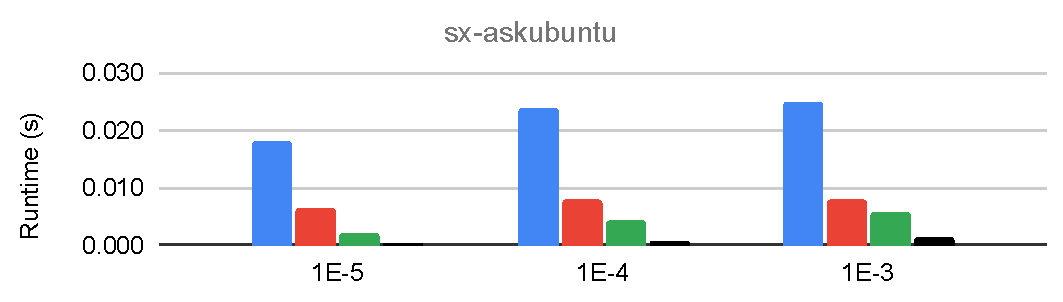
\includegraphics[width=0.48\linewidth]{out/temporal-summary-runtime-sx-askubuntu.pdf}
  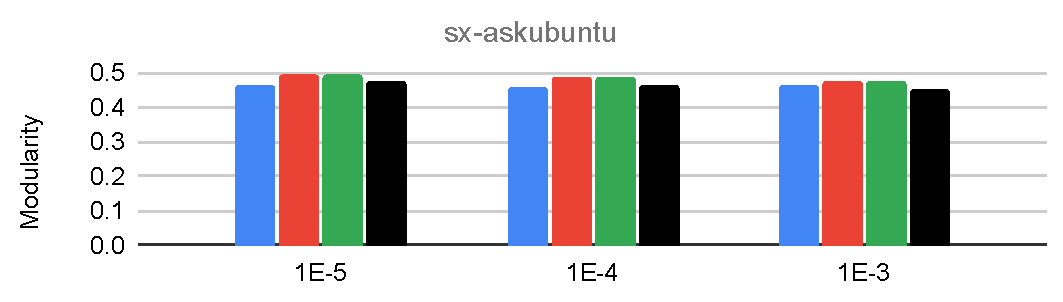
\includegraphics[width=0.48\linewidth]{out/temporal-summary-modularity-sx-askubuntu.pdf}
  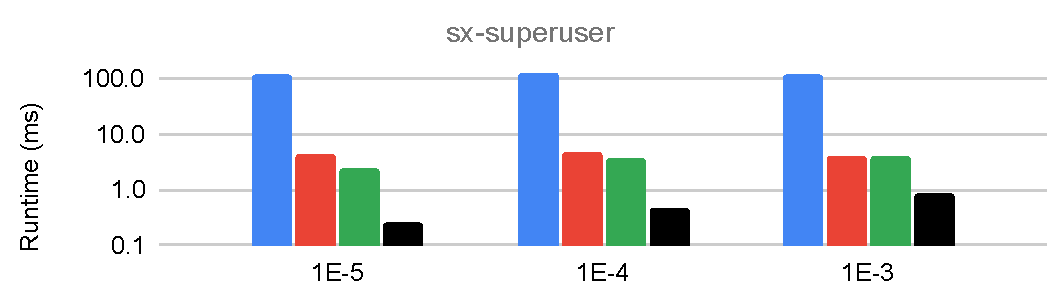
\includegraphics[width=0.48\linewidth]{out/temporal-summary-runtime-sx-superuser.pdf}
  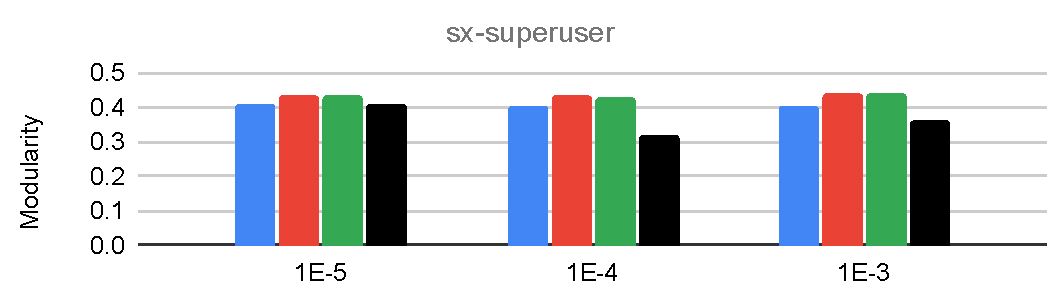
\includegraphics[width=0.48\linewidth]{out/temporal-summary-modularity-sx-superuser.pdf}
  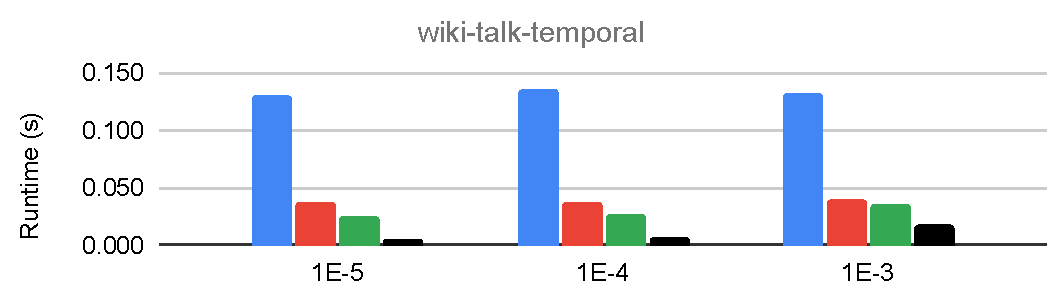
\includegraphics[width=0.48\linewidth]{out/temporal-summary-runtime-wiki-talk-temporal.pdf}
  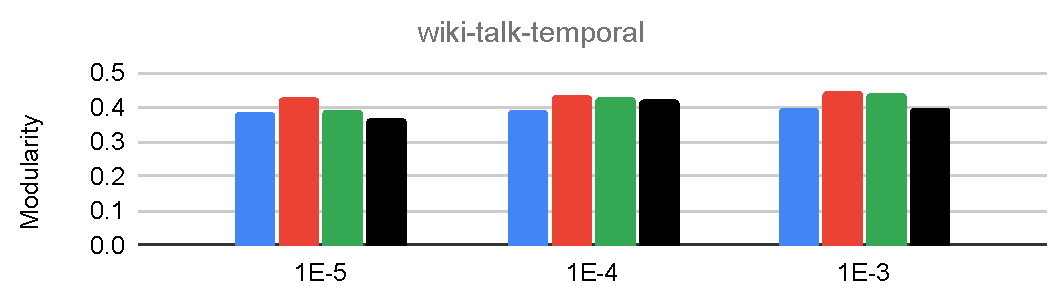
\includegraphics[width=0.48\linewidth]{out/temporal-summary-modularity-wiki-talk-temporal.pdf}
  \subfigure[Runtime on each dynamic graph]{
    \label{fig:temporal-summary--runtime-graph}
    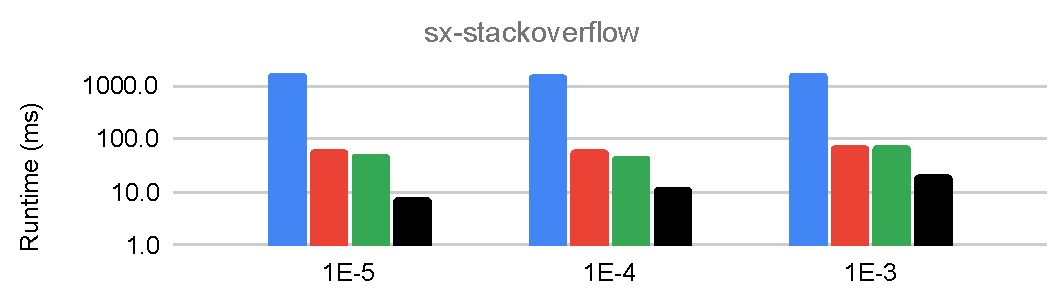
\includegraphics[width=0.48\linewidth]{out/temporal-summary-runtime-sx-stackoverflow.pdf}
  }
  \subfigure[Modularity in communities obtained on each dynamic graph]{
    \label{fig:temporal-summary--modularity-graph}
    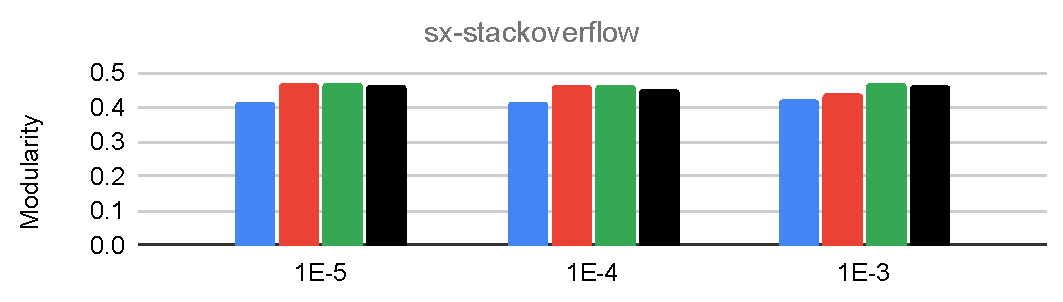
\includegraphics[width=0.48\linewidth]{out/temporal-summary-modularity-sx-stackoverflow.pdf}
  } \\[-2ex]
  \caption{Mean Runtime and Modularity of communities obtained with our GPU implementation of \textit{Static}, \textit{Naive-dynamic (ND)}, \textit{Dynamic Traversal (DT)}, \textit{Dynamic Frontier (DF)}, and \textit{Dynamic Frontier with Pruning (DF-P)} PageRank on real-world dynamic graphs, with batch updates of size $10^{-5}|E_T|$ to $10^{-3}|E_T|$. Here, (a) and (b) show the overall runtime and modularity across all temporal graphs, while (c) and (d) show the runtime and rank modularity for each approach (relative to reference Static PageRank, see Section \ref{sec:measurement}). In (a), the speedup of each approach with respect to Static PageRank is labeled.}
  \label{fig:temporal-summary}
\end{figure*}

\begin{figure*}[hbtp]
  \centering
  \subfigure[Overall result]{
    \label{fig:8020-runtime--mean}
    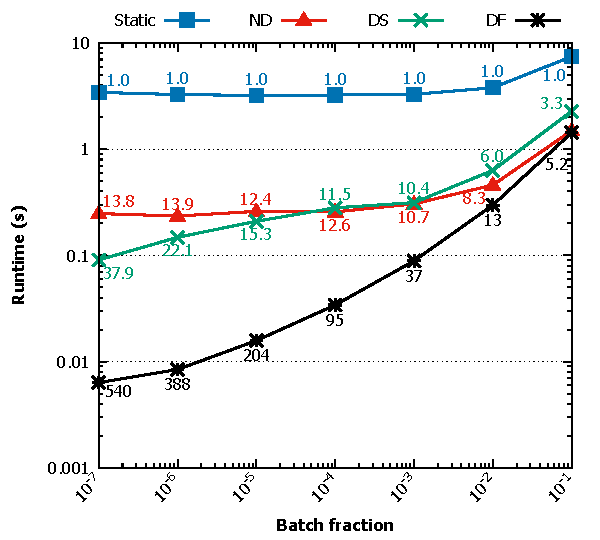
\includegraphics[width=0.38\linewidth]{out/8020-runtime-mean.pdf}
  }
  \subfigure[Results on each graph]{
    \label{fig:8020-runtime--all}
    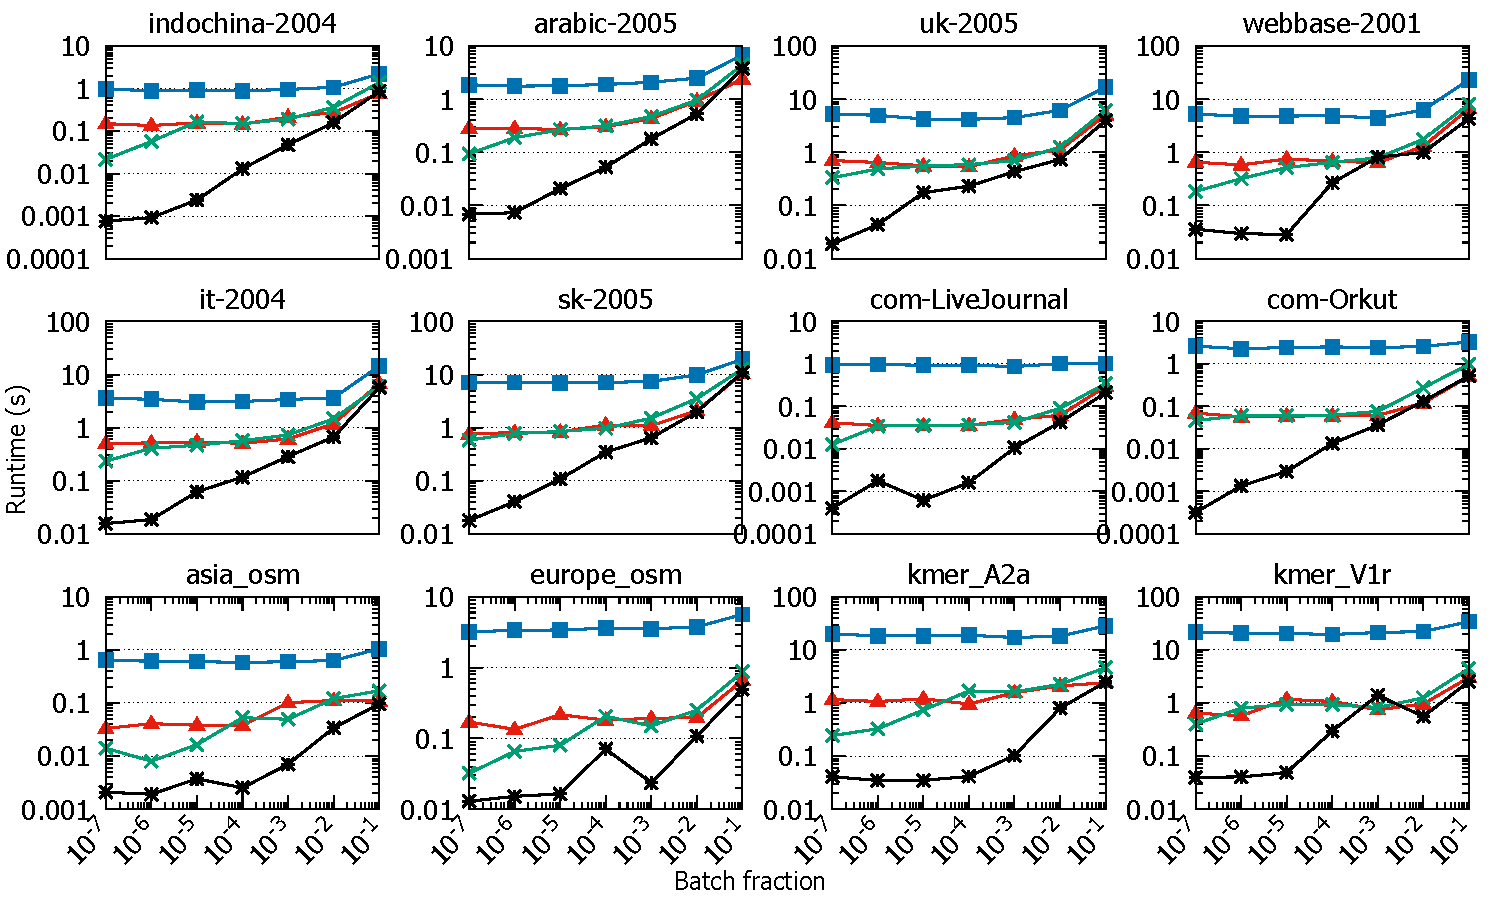
\includegraphics[width=0.58\linewidth]{out/8020-runtime-all.pdf}
  } \\[-2ex]
  \caption{Runtime (logarithmic scale) of our multicore implementation of \textit{Static}, \textit{Naive-dynamic (ND)}, \textit{Delta-screening (DS)}, and \textit{Dynamic Frontier (DF)} Louvain on large (static) graphs with generated random batch updates. Batch updates range in size from $10^{-7}|E|$ to $0.1|E|$ in multiples of $10$. These updates consist of $80\%$ edge insertions and $20\%$ edge deletions, mimicking realistic changes in a dynamic graph scenario. The right subfigure illustrates the runtime of each approach for individual graphs in the dataset, while the left subfigure presents overall runtimes (using geometric mean for consistent scaling across graphs). Additionally, the speedup of each approach relative to Static Louvain is labeled on respective lines.}
  \label{fig:8020-runtime}
\end{figure*}

\begin{figure*}[hbtp]
  \centering
  \subfigure[Overall result]{
    \label{fig:8020-modularity--mean}
    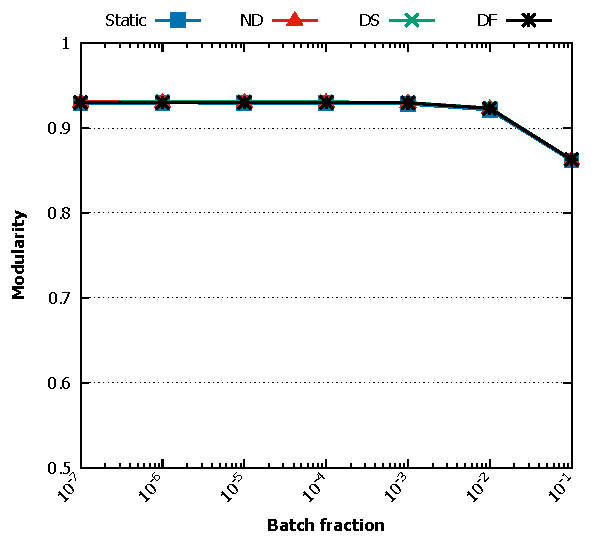
\includegraphics[width=0.38\linewidth]{out/8020-modularity-mean.pdf}
  }
  \subfigure[Results on each graph]{
    \label{fig:8020-modularity--all}
    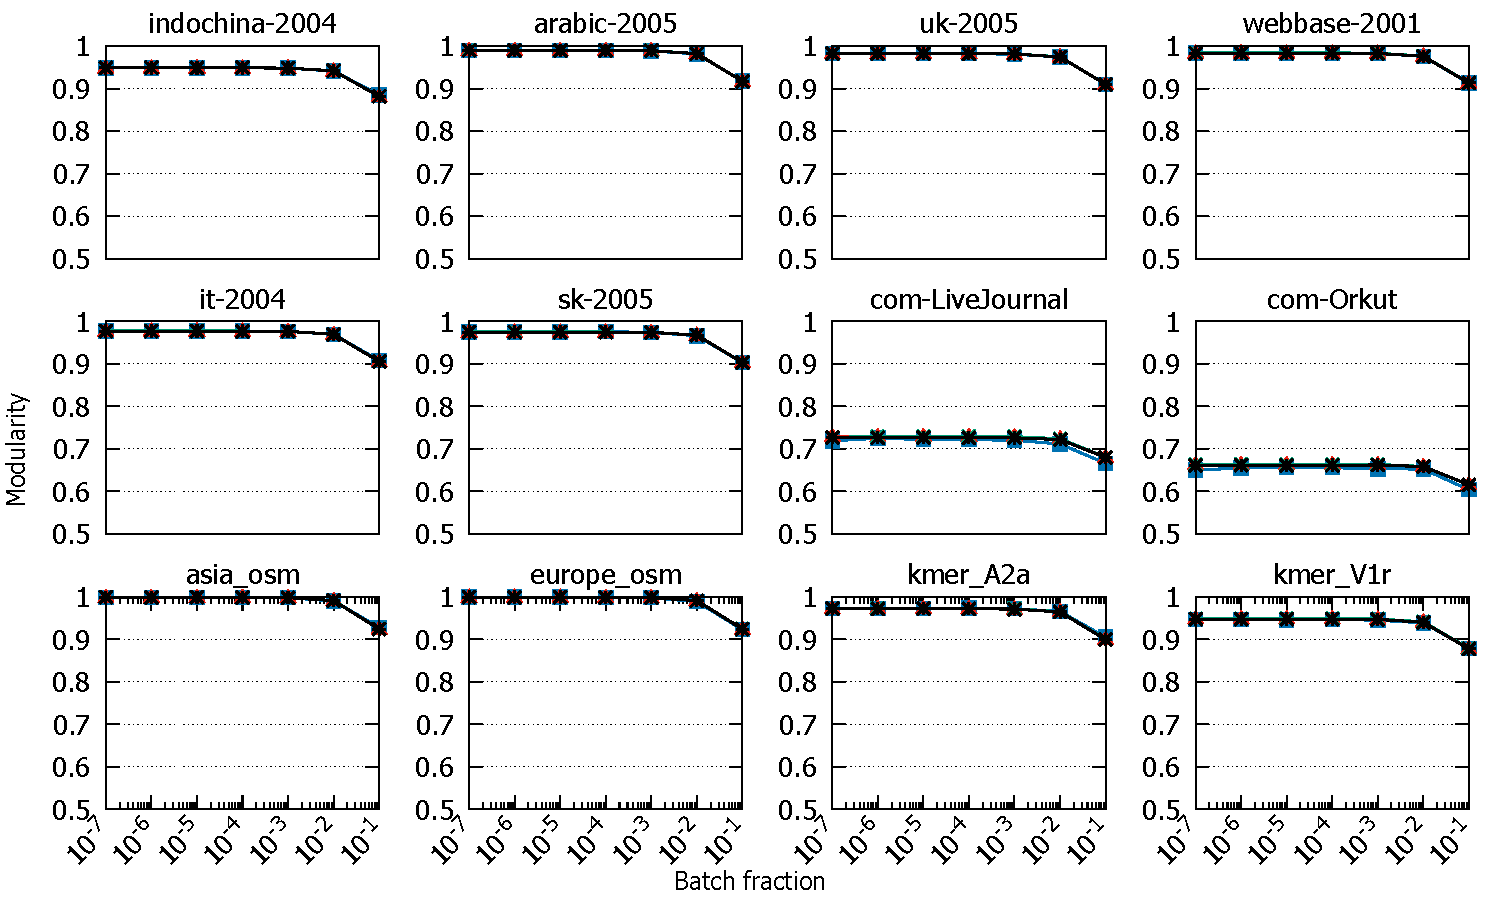
\includegraphics[width=0.58\linewidth]{out/8020-modularity-all.pdf}
  } \\[-1ex]
  \caption{Modularity comparison of our GPU implementation of \textit{Static}, \textit{Naive-dynamic (ND)}, \textit{Dynamic Traversal (DT)}, \textit{Dynamic Frontier (DF)}, and \textit{Dynamic Frontier with Pruning (DF-P)} PageRank on large (static) graphs with generated random batch updates, relative to a Reference Static PageRank (see Section \ref{sec:measurement}), using $L1$-norm. The size of batch updates range from $10^{-7} |E|$ to $0.1 |E|$ in multiples of $10$ (logarithmic scale), consisting of $80\%$ edge insertions and $20\%$ edge deletions to simulate realistic dynamic graph updates. The right subfigure depicts the modularity for each approach in relation to each graph, while the left subfigure showcases overall modularitys using geometric mean for consistent scaling across graphs.}
  \label{fig:8020-modularity}
\end{figure*}



\ignore{\subsubsection{Determining optimality of result}}
\ignore{\label{sec:evaluation--optimality}}

\ignore{Community detection is an NP-hard problem and existing polynomial algorithms are \textit{heuristic}. We study correctness in terms of \textit{modularity score} of communities identified (higher is better), similar to previous works in the area \cite{com-traag19, com-zarayeneh21}. As Figures \ref{fig:louvain}-\ref{fig:hybrid} show, modularity of communities detected by our proposed dynamic algorithms is close to the modularity of communities detected by corresponding static algorithms.}

\begin{figure*}[hbtp]
  \centering
  \subfigure[Dynamic Louvain algorithms]{
    \label{fig:measure-affected--temporal}
    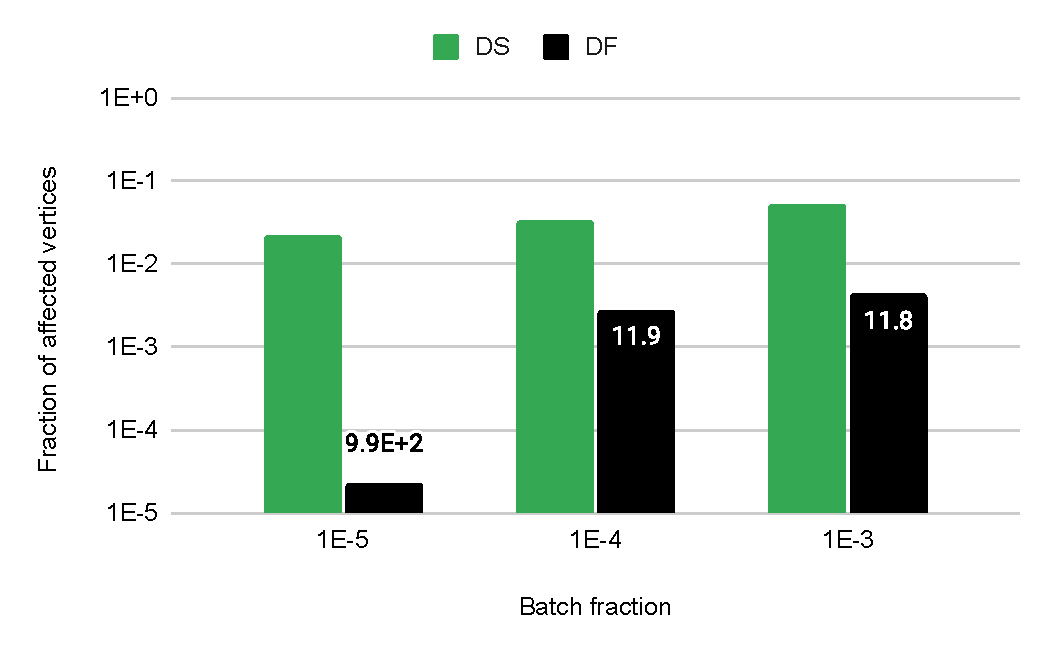
\includegraphics[width=0.48\linewidth]{out/measure-affected-temporal.pdf}
  }
  \subfigure[Dynamic LPA algorithms]{
    \label{fig:measure-affected--8020}
    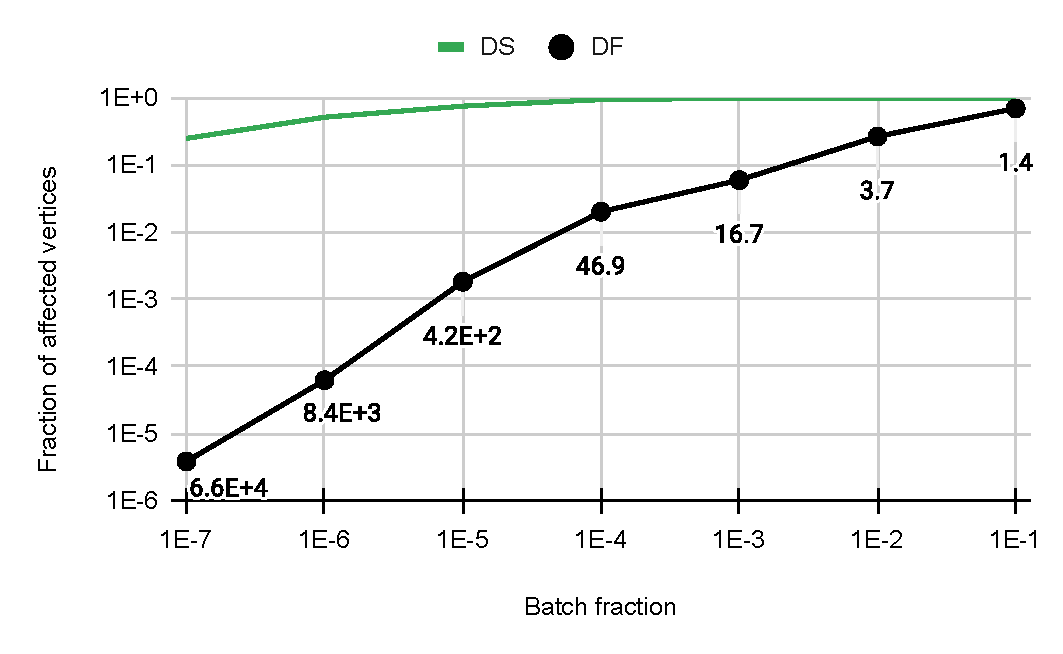
\includegraphics[width=0.48\linewidth]{out/measure-affected-8020.pdf}
  } \\[-2ex]
  \caption{Mean percentage of vertices marked as affected by \textit{Delta-screening (DS)} and our \textit{Dynamic Frontier (DF)} Louvain, on real-world dynamic graphs (with batch updates of size $10^{-5}|E|$ to $10^{-3}|E|$), and on large graphs with random batch updates ($80\%$ insertions, $20\%$ deletions with batch updates of size $10^{-7}|E|$ to $0.1|E|$).}
  \label{fig:measure-affected}
\end{figure*}

\ignore{\begin{figure}[hbtp]
  \centering
  \subfigure{
    \label{fig:measure-stability--5050}
    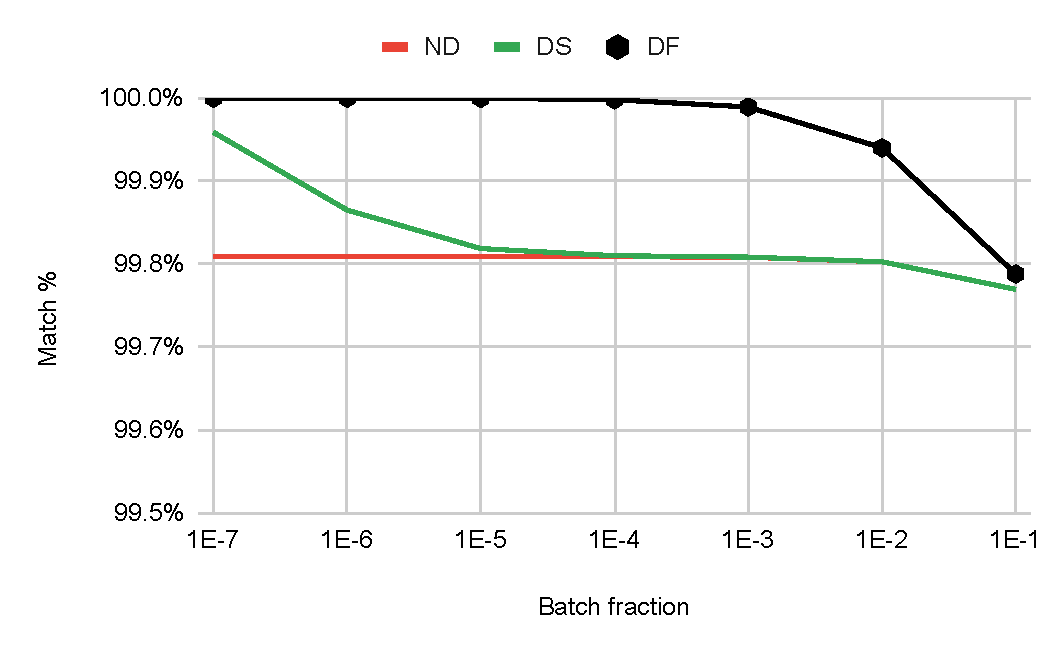
\includegraphics[width=0.98\linewidth]{out/measure-stability-5050.pdf}
  } \\[-2ex]
  \caption{Test.}
  \label{fig:measure-stability}
\end{figure}
}




\subsection{Performance Comparison}
\label{sec:performance-comparison}

\subsubsection{Results on real-world dynamic graphs}

We now compare the performance of our Parallel Dynamic Frontier (DF) Louvain with our parallel implementation of Static, Naive-dynamic (ND), and Delta-screening (DS) Louvain on real-world dynamic graphs from Table \ref{tab:dataset}. These evaluations are conducted on batch updates of size $10^{-5}|E_T|$ to $10^{-3}|E_T|$ in multiples of $10$. For each batch size, as mentioned in Section \ref{sec:batch-generation}, we load $90\%$ of the graph, add reverse edges to make all edges in the graph undirected, and then load $B$ edges (where $B$ is the batch size) consecutively in $100$ batch updates. The work of Zarayeneh et al. \cite{com-zarayeneh21} demonstrates improved performance of the DS approach compared to DynaMo \cite{com-zhuang19} and Batch \cite{com-chong13}. Thus, we limit our comparison to DS Louvain. Figure \ref{fig:temporal-summary--runtime-overall} displays the overall runtime of each approach across all graphs for each batch size, while Figure \ref{fig:temporal-summary--modularity-overall} illustrates the overall modularity of obtained communities. Additionally, Figures \ref{fig:temporal-summary--runtime-graph} and \ref{fig:temporal-summary--modularity-graph} present the mean runtime and modularity of communities obtained with the approaches on each dynamic graph in the dataset. Finally, Figures \ref{fig:temporal-sx-mathoverflow}, \ref{fig:temporal-sx-askubuntu}, \ref{fig:temporal-sx-superuser}, \ref{fig:temporal-wiki-talk-temporal}, and \ref{fig:temporal-sx-stackoverflow} show the runtime and modularity of communities obtained with Static, ND, DS, and DF Louvain on each dynamic graph in Table \ref{tab:dataset}, upon each consecutive batch update.

Figure \ref{fig:temporal-summary--runtime-overall} shows that DF Louvain is, on average, $268\times$, $195\times$, and $109\times$ faster than Static Louvain on batch updates of size $10^{-5}|E_T|$, $10^{-4}|E_T|$, and $10^{-3}|E_T|$, respectively. In contrast, DS Louvain demonstrates average speedups of $47\times$, $32\times$, and $26\times$ over Static Louvain for batch update sizes of $10^{-5}|E_T|$ to $10^{-3}|E_T|$, while ND Louvain obtains a mean speedup of $25\times$\ignore{over Static Louvain}.\ignore{DF Louvain thus achieves average speedups of $5.7\times$, $6.1\times$, and $4.2\times$ compared to DS Louvain for the same batch updates.} DF Louvain is thus, overall, $179\times$, $7.2\times$, and $5.3\times$ faster than Static, ND, and DS Louvain. This speedup is particularly pronounced on the \textit{sx-superuser} graph, as indicated by Figure \ref{fig:temporal-summary--runtime-graph}. Regarding modularity, Figures \ref{fig:temporal-summary--modularity-overall} and \ref{fig:temporal-summary--modularity-graph} illustrate that DF Louvain generally exhibits slightly lower modularity on average compared to ND and DS Louvain but is on par with the modularity obtained by Static Louvain, except for the \textit{sx-superuser} graph (because it fails to mark certain vertices as affected, likely because they are outlier vertices and were not directly reached from the expanding frontier). This makes the communities obtained with DF Louvain generally acceptable. However, if lower modularity is observed (during intermediate empirical tests), transitioning to our parallel implementation of DS Louvain is advisable. It is also worth noting that ND Louvain produces higher-quality communities than Static Louvain, as it builds upon the community memberships obtained from Static Louvain and further optimizes them (we limit the number of passes for Static Louvain to achieve a large speed gain, even if it means sacrificing some quality).


\subsubsection{Results on large graphs with random batch updates}

We also assess the performance of our parallel DF Louvain alongside our parallel implementation of Static, ND, and DS Louvain on large (static) graphs listed in Table \ref{tab:dataset-large}, with randomly generated batch updates. As elaborated in Section \ref{sec:batch-generation}, the batch updates vary in size from $10^{-7}|E|$ to $0.1|E|$ (in multiples of $10$), comprising $80\%$ edge insertions and $20\%$ edge deletions to mimic realistic scenarios. Reverse edges are added with each batch update, to ensure that the graph is undirected. As mentioned in Section \ref{sec:batch-generation}, we generate $5$ different random batch updates for each batch size to minimize measurement noise. Figure \ref{fig:8020-runtime} illustrates the runtime of Static, ND, DS, and DF Louvain, while Figure \ref{fig:8020-modularity} displays the modularity of communities obtained with each approach.

Figure \ref{fig:8020-runtime--mean} illustrates that DF Louvain achieves a mean speedup of $183\times$, $13.8\times$, and $8.7\times$ compared to Static, ND, and DS Louvain, respectively. On a batch update of size $10^{-7}|E|$, DF Louvain is significantly faster, attaining speedups of $540\times$, $39\times$, and $14\times$, with respect to Static, ND, and DS Louvain, respectively. The speedup is particularly pronounced on web graphs, social networks, and protein k-mer graphs, characterized by a large number of vertices (as depicted in Figure \ref{fig:8020-runtime--all}). It may be noted that DS Louvain exhibits slower performance than ND Louvain on large batch updates, i.e., on batch updates of size $0.01|E|$ and $0.1|E|$. This is attributed to the cost of initial marking of affected vertices with DS Louvain --- since the updates are scattered randomly across the graph, DS Louvain ends up marking a significant number of vertices as affected, making it almost equivalent to ND Louvain, but with the added cost of the marking of affected vertices (particularly on web graphs and social networks, characterized by a high average degree and a small diameter). Figures \ref{fig:8020-modularity--mean} and \ref{fig:8020-modularity--all} indicate that DF Louvain obtains communities with the roughly same modularity as Static, ND, and DS Louvain. Hence, for large graphs with random batch updates, DF Louvain is the best dynamic community detection method.

In Figure \ref{fig:8020-runtime}, also note that runtime of Static Louvain increases for larger batch updates. This more likely due to the random batch updates arbitrarily disrupting the original community structure --- which results in Static Louvain needing more iterations to converge --- than due to the increased number of edges in the graph.


\subsubsection{Comparison of vertices marked as affected}

Figure \ref{fig:measure-affected--temporal} displays the mean percentage of vertices marked as affected by DS and DF Louvain on real-world dynamic graphs from Table \ref{tab:dataset}, with batch updates of size $10^{-5}|E_T|$ to $10^{-3}|E_T|$ in multiples of $10$ (see Section \ref{sec:batch-generation} for details) --- while Figure \ref{fig:measure-affected--8020} displays the mean percentage of vertices marked as affected by DS and DF Louvain on large (static) graphs with generated random batch updates (consisting of $80\%$ edge insertions and $20\%$ deletions), on batch updates of size $10^{-7}|E|$ to $0.1|E|$. For DS Louvain, the affected vertices are marked at the start of the algorithm, while, for DF Louvain, affected vertices are marked incrementally --- therefore, we count all vertices that were ever flagged as affected with DF Louvain.

Figure \ref{fig:measure-affected--temporal} shows that the proportion of vertices marked as affected by DF Louvain is $990\times$, $11.9\times$, and $11.8\times$ lower than DS Louvain for batch updates of size $10^{-5}|E_T|$, $10^{-4}|E_T|$, and $10^{-3}|E_T|$, respectively. Figure \ref{fig:measure-affected--8020} also paints a similar picture, with significantly fewer vertices being marked as affected by DF Louvain for smaller batch updates (i.e., batch updates of size $10^{-7}|E|$ and $10^{-6}|E|$). Therefore, the performance improvement with DF Louvain can be attributed to both marking fewer vertices as affected, and to the incremental marking of affected vertices. Additionally, it is worth noting that, on real-world dynamic graphs, the fraction of vertices marked as affected is generally low across both approaches. This is likely because updates in such graphs tend to be concentrated in specific regions of the graph\ignore{(not randomly scattered throughout)}.


\ignore{\subsubsection{Stability}}
\ignore{\label{sec:stability}}

\ignore{Intuitively, if the graphs $G^t$ and $G^{t'}$ are identical for some $t$ and $t'$, we expect DF Louvain to produce the same communities for $G^t$ and $G^{t'}$. We refer to this property of a dynamic algorithm as its stability, measured as the percentage of vertices that agree on the community label across two identical graphs. Vertices within weak community structures tend to be unstable, as they may connect to multiple communities with similar strength.}

\ignore{To measure the stability of ND, DS, and DF Louvain, we proceed as follows. Let $G$ be an initial graph. We generate random batch updates of size $10^{-7} |E|$ to $0.1 |E|$ consisting of edge deletions to obtain the graph $G^1$. We then apply each of the above algorithms on $G^1$ to identify the new communities. Subsequently, we create another batch of updates that consists of inserting the edges deleted in the prior time step. This graph, $G^2$, is essentially the original graph $G$. We obtain the community labels of the vertices in the graph $G^2$ by appealing to the dynamic algorithms. Finally, we compare the community label of each vertex in the graphs $G$ and $G^2$. The resulting match in community membership of vertices with ND, DS, and DF Louvain on batch updates of size $10^{-7} |E|$ to $0.1 |E|$ is shown in Figure \ref{fig:louvainrak-stability--louvain}.}

\ignore{From Figure \ref{fig:louvainrak-stability--louvain}, we observe that ND and DS Louvain have minimum of $99.68\%$ match with the original community memberships across all batch sizes, while DF Louvain has a minimum of $99.70\%$ match. This indicates that all these algorithms are stable.}

\begin{figure}[!hbt]
  \centering
  % \subfigure{
  %   \label{fig:strong-scaling--temporal}
  %   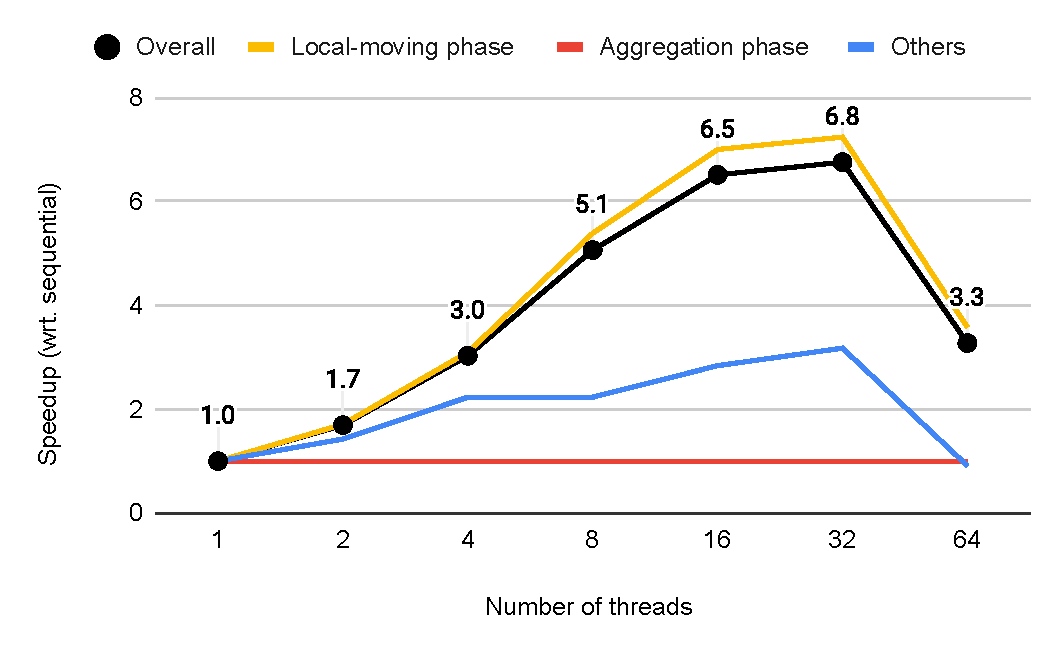
\includegraphics[width=0.98\linewidth]{out/strong-scaling-temporal.pdf}
  % }
  \subfigure{
    \label{fig:strong-scaling--8020}
    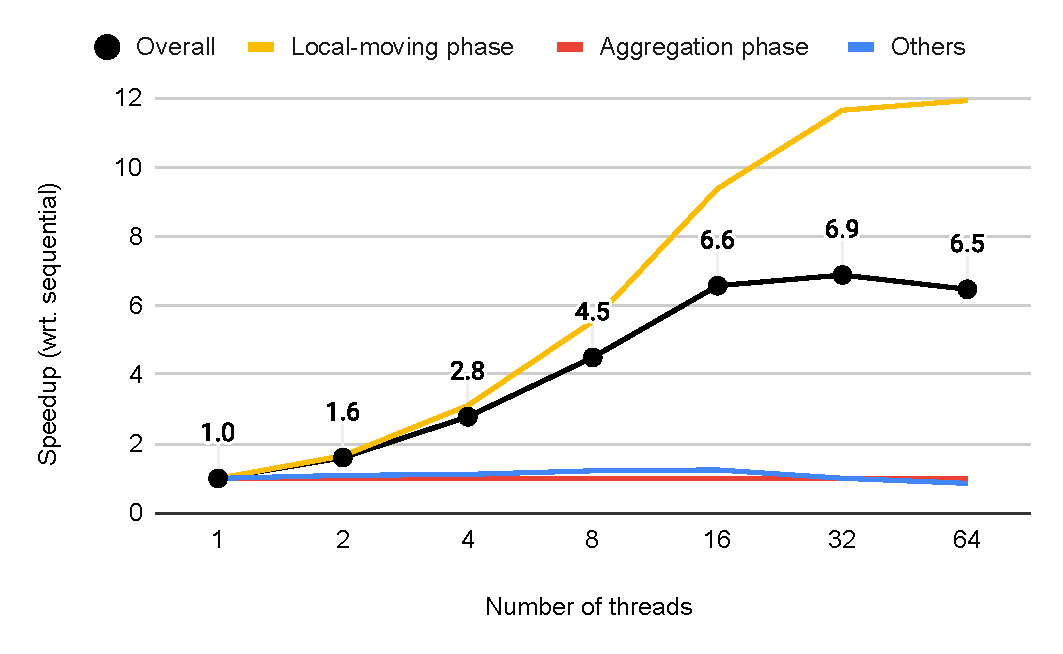
\includegraphics[width=0.98\linewidth]{out/strong-scaling-8020.pdf}
  } \\[-2ex]
  \caption{Mean speedup of\ignore{our} \textit{Dynamic Frontier (DF)} Louvain with increasing number of threads (in multiples of $2$), on large\ignore{(static)} graphs with random batch updates of size $10^{-7}|E|$ to $0.1|E|$, composed $80\%$ edge insertions and $20\%$ insertions.}
  \label{fig:strong-scaling}
\end{figure}



\subsubsection{Strong scaling}
\label{sec:strong-scaling}

Finally, we study the strong-scaling behavior of DF Louvain on large (static) graphs, with generated random batch updates of size $10^{-7}|E|$ to $0.1|E|$. The speedup of DF Louvain is measured as the number of threads increases from $1$ to $64$ in multiples of $2$, relative to single-threaded execution. This process is repeated for each graph in the dataset (refer to Table \ref{tab:dataset}), and the results are averaged using geometric mean.

The results, depicted in Figure \ref{fig:strong-scaling}, indicate that with $16$ threads, DF Louvain achieves an average speedup of $6.6\times$ compared to single-threaded execution, showing a performance increase of $1.6\times$ for every doubling of threads. The speedup of DF Louvain is lower, likely due to the reduced work performed by the algorithm. At $32$ and $64$ threads, DF Louvain is affected by NUMA effects (the $64$-core processor used has $4$ NUMA domains), resulting in a speedup of only $6.9\times$ and $6.5\times$, respectively. The results are similar on real-world dynamic graphs\ignore{, as shown in Figure X}, but the speedup is even lower for $64$ threads to due lack of sufficient work per thread.
